\documentclass{classrep}
\usepackage[utf8]{inputenc}
\frenchspacing

\usepackage{graphicx}
\usepackage[usenames,dvipsnames]{color}
\usepackage[hidelinks]{hyperref}
\usepackage{subfig}

\usepackage{amsmath, amssymb, mathtools}

\usepackage{fancyhdr, lastpage}
\pagestyle{fancyplain}
\fancyhf{}
\renewcommand{\headrulewidth}{0pt}
\cfoot{\thepage\ / \pageref*{LastPage}}


\studycycle{Informatyka, studia dzienne, I st.}
\coursesemester{IV}

\coursename{Inteligentna Analiza Danych}
\courseyear{2016/2017}

\courseteacher{mgr inż. Paweł Tarasiuk}
\coursegroup{piątek, 12:00}

\author{%
  \studentinfo[203943@edu.p.lodz.pl]{Jakub Mielczarek}{203943}\\
  \studentinfo[203882@edu.p.lodz.pl]{Łukasz Gołębiewski}{203882}%
}

\title{Zadanie 1.: Samoorganizujące mapy neuronowe z wykorzystaniem algorytmów: Kohonena, gazu neuronowego, k-średnich}

\begin{document} 
\maketitle 
\thispagestyle{fancyplain}

\section{Cel}
{\color{black}
Przedmiotem zadania jest implementacja algorytmów służących do przetwarzania zbiorów danych i ich klasyfikacji (grupowania) na mniejsze podzbiory według ściśle określonych zasad.

\section{Wprowadzenie}
{\color{black}
Zadanie zostało podzielone na trzy warianty i w ten sposób zaprezentujemy teorię niezbędną do jego realizacji.

\subsection*{Wariant I: Kwantyzacja przestrzeni za pomocą samoorganizującej się sieci neuronowej przy pomocy algorytmu Kohonena oraz algorytmu gazu neuronowego}
Mamy zbiór danych opisujących punkty dla przestrzeni o dowolnej liczbie wymiarów. Pierwszym krokiem algorytmu Kohonena jest wygenerowanie neuronów, względem których będziemy dokonywać klasyfikacji. Neurony generujemy losowo wykorzystując rozkład Gaussa parametryzowany poprzez obliczenie średniej arytmetycznej oraz odchylenia standardowego dla punktów i-tego wymiaru. Neurony są losowane kilka razy wybierając tą strukturę która ma najmniej martwych neuronów. Średnia arytmetyczna: 
\begin{equation}
\sqrt{\dfrac{\sum_{i=1}^{n} x_i}{n} }
\end{equation}
Odchylenie standardowe:
\begin{equation}
\sqrt{\dfrac{\sum_{i=1}^{n} {(x_i - \bar{x})^2}}{n} }
\end{equation}
Odległość euklidesowa:
\begin{equation}
\sqrt{\dfrac{\sum_{i=1}^{n} {(x_{iA} - x_{iB})^2}}{n} }
\end{equation}
Kolejnym etapem jest przyporządkowanie do każdego punktu najbliższego mu neuronu(3). Wynik tej operacji jest zapisywany jako lista indeksów odpowiadających indeksom w liście neuronów. Następnie przechodzimy do najistotniejszej części algorytmu. Wybieramy losowy punkt oraz przyporządkowany mu neuron. Neuron ten od tego momentu będziemy określać jako "zwycięzcę" (BMU). Następnie obliczamy wagi (nowe współrzędne) wszystkich neuronów korzystając z następujących wzorów: 
\begin{equation}
learningRate=learningRate_0 * exp(\dfrac{-i}{numberOfIterations})
\end{equation}
\begin{equation}
timeConst=\dfrac{numberOfIterations}{(mapRadius_0 * timeConst_0)}
\end{equation}
\begin{equation}
mapRadius=mapRadius_0 * exp(\dfrac{-i}{timeConst})
\end{equation}
\begin{equation}
influence=exp(\dfrac{-(distFromBMU)^2}{2*(mapRadius)^2})
\end{equation}
\begin{equation}
w_{ij}(new)=w_{ij}(old)+learningRate  * influence *  (x_j - w_{ij}(old) )
\end{equation}
Podany powyżej wzór (7) wykorzystuje gaussowską funkcję sąsiedztwa.
Należy zauważyć, że również neurony-sąsiedzi podlegają modyfikacji, jednakże w słabszym stopniu. Algorytm jest powtarzany do osiągnięcia kryterium zbieżności, którym w tym przypadku jest liczba iteracji. Algorytm gazu neuronowego działa analogicznie jak algorytm Kohonena, przy czym zagadnienie sąsiedztwa rozwiązane jest przez uporządkowanie neuronów w szereg w zależności od odległości ich wektorów wagowych od podanego wektora wejściowego. Współczynnik nauki wyznaczany jest w tym przypadku na podstawie pozycji w szeregu, a nie faktycznej odległości(pozycja w szeregu jest ustalana poprzez odległość od BMU w kolejności rosnącej):
\begin{equation}
influence=exp(\dfrac{-(i)^2}{2*(mapRadius)^2})
\end{equation}

\subsection*{Wariant II: Kwantyzacja przestrzeni za pomocą samoorganizującej się sieci neuronowej przy pomocy algorytmu k-średnich}
Mamy zbiór danych opisujących punkty dla przestrzeni o dowolnej liczbie wymiarów. Pierwszym krokiem algorytmu jest wygenerowanie centroidów (klas), względem których będziemy dokonywać klasyfikacji. Centroidy generujemy losowo wykorzystując rozkład Gaussa parametryzowany poprzez obliczenie średniej arytmetycznej(1) oraz odchylenia standardowego(2) dla punktów i-tego wymiaru. Neurony są losowane kilka razy wybierając tą strukturę która ma najmniej martwych neuronów. Kolejnym etapem jest obliczenie odległości punktów od centroidów i przypisanie ich do najbliższego k-centroidu(3). Ostatnim krokiem jest obliczenie średniej arytmetycznej(1) punktów należących do danego klastra. Jej wartość to nowe współrzędne k-centroidu. Algorytm jest powtarzany aż do osiągnięcia warunku kończącego. W naszej implementacji jest to określona z góry liczba iteracji lub otrzymanie tych samych współrzędnych dla centroidów w i+1 kroku iteracji.

\subsection*{Wariant III: Kompresja obrazu}
Aby skompresować obraz za pomocą w/w algorytmów najpierw przygotowujemy dane RGB pikseli z obrazu do pliku tekstowego. Obrazek jest dzielony na kwadratowe ramki o boku równym ilości pikseli zadanej przez użytkownika. Następnie każda ramka przekształcana jest do pliku tekstowego w taki sposób, że reprezentuje jedną daną. Dla przykładu dla kolorowego obrazka dla ramki o boku 3 pikseli jedna ramka będzie reprezentowana jako punkt w przestrzeni 27-wymiarowej - każdy piksel ma jeszcze 3 składowe RGB. Po zakończeni działania wybranego algorytmu należy jeszcze zastąpić wartości każdej ranki przyporządkowanym jej neuronem. Na sam koniec przeprowadza się operację zapisania przekształconych ramek do obrazka o wybranym formacie. 

\section{Opis implementacji}
Podstawowy opis plików klas:
\begin{itemize}
	\item Neural.java \ppauza klasa abstrakcyjna zawierające wspólne pola i metody dla każdego z algorytmów. 
	\begin{itemize}
		\item Kohonen.java \ppauza implementacja algorytmu SOM Kohonena.
		\item NeuralGas.java \pauza implementacja algorytmu gazu neuronowego.
		\item KMeans.java \ppauza implementacja algorytmu k-średnich. 
	\end{itemize}
	\item FileHandler.java \ppauza klasaa zawierająca statyczne metody do działań związanych z operacjami na plikach np. zapis macierzy danych do pliku w odpowiednim formacie tabulacji i znaków nowej linii. Odczyt danych z obrazu, zamiana pikseli z obrazka na ramki i zapis ich do pliku itp.  
	\item Utils.java \ppauza klasa pomocnicza zawierająca statyczne metody do operacji takich jak normalizacja danych, pobranie wybranej kolumny z podanej struktury danych w postaci macierzy itp.
	\item DataMath.java \ppauza klasa pomocnicza zawierająca statyczne metody do obliczania średnich, median, odchyleń standardowych itp.
	\item Metric.java \ppauza klasa pomocnicza zawierająca statyczne metody do obliczania odległości pomiędzy punktami n-wymiarowymi w wybranej metryce.
\end{itemize}
Program, który wykorzystaliśmy do rysowania wykresów to Gnuplot. Odpowiednie pliki zawierające skrypty są wywoływane w trakcie działania programu co pozwala na odczyt danych w czasie rzeczywistym.
Warto zauważyć, że przygotowane klasy posiadają dość duża ilość parametrów. Parametry pozwalają na:
\begin{itemize}
	\item ustalenie wszystkich początkowych wartości parametrów dla każdego algorytmu.
	\item podanie ścieżki do pliku z danymi
	\item ustalenie czy chcemy aby program generował wykresy. Jeśli nie, 
oszczędzamy wówczas na dość kosztownych pod względem czasowym operacji na plikach podczas iteracji algorytmu (program nie musi przygotowywać plików dla gnuplota). 
\end{itemize}

\section{Materiały i metody}
{
Dla każdego algorytmu podawana jest ilość iteracji, ilość centroidów(neuronów), plik źródłowy z danymi oraz dodatkowo dla algorytmów kohonena oraz gazu neuronowego wartości odpowiednich współczynników wpływających na przebieg oraz rezultat obliczeń. Dyskusji wyników dokonamy sprawdzając zachowania algorytmów dla określonych danych wejściowych i porównując je ze sobą. Przedstawimy również skrajne przypadki, które wpływają na nieefektywność zastosowanych rozwiązań. }

\section{Wyniki}
{

\begin{figure}[h!]
 \centering
 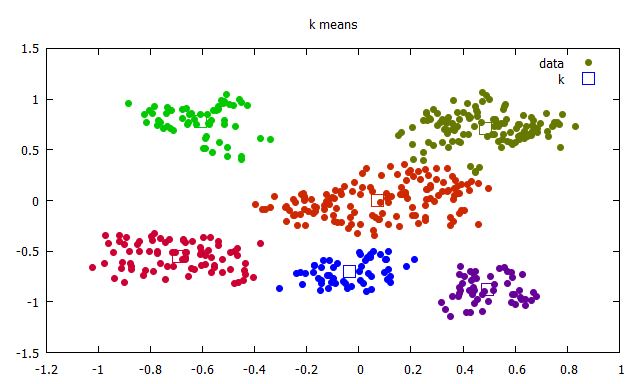
\includegraphics[width=12cm]{img/kmeanssample1_6_10.png}
 \vspace{-0.3cm}
 \caption{Data: sample1 Algorytm: k-średnich n = 6 iter = 10  }
\end{figure}
 
 
\begin{figure}[h!]
 \centering
 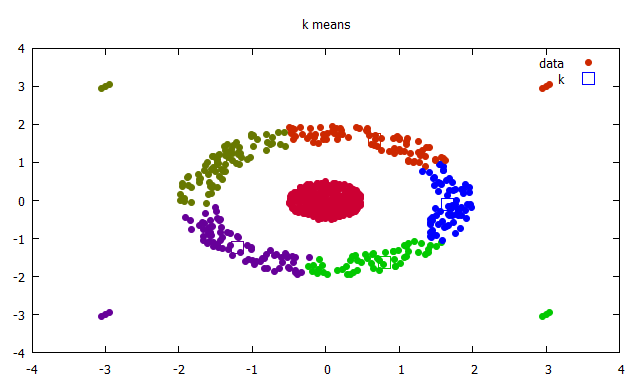
\includegraphics[width=12cm]{img/kmeanscircle1_6_10.png}
 \vspace{-0.3cm}
 \caption{Data: circle1 Algorytm: k-średnich n = 6 iter = 10  }
\end{figure}

\newpage


\begin{figure}[h!]
\centering
 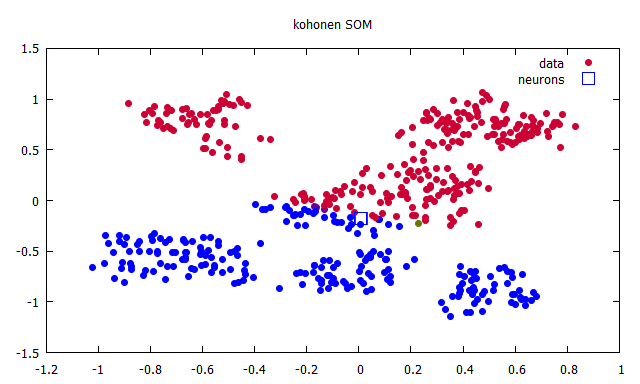
\includegraphics[width=12cm]{img/kohonensample1_6_1000.png}
 \vspace{-0.3cm}
 \caption{Data: sample1 Algorytm: kohonena n = 6 iter = 1000
  mapRadius = 1 learningRate = 0.1 learningRate0 = 1  
}
\end{figure}

\newpage

\begin{figure}[h!]
\centering
 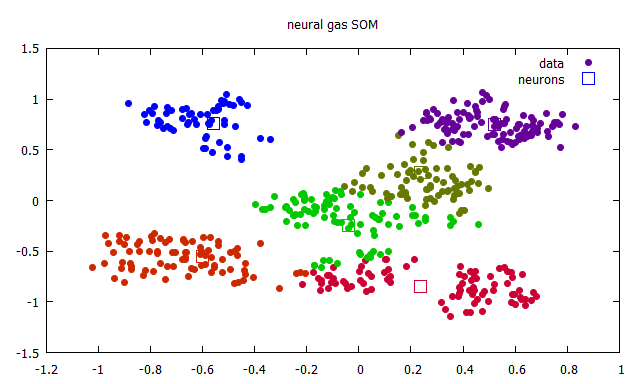
\includegraphics[width=12cm]{img/neuralsample1_6_1000.png}
 \vspace{-0.3cm}
 \caption{Data: circle1 Algorytm: gazu neuronowego n = 6 iter = 1000
  mapRadius = 1 learningRate = 0.1 learningRate0  = 1  
}
\end{figure}

\begin{figure}[h!]
\centering
 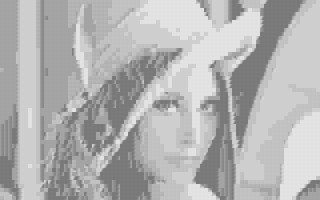
\includegraphics[width=12cm]{img/kmeans_1.png}
 \vspace{-0.0cm}
 \caption{Data: lena Algorytm: k-średnich frameSz = 4 n = 10 iter = 10
}
\end{figure}

\newpage

\begin{figure}[h!]
\centering
 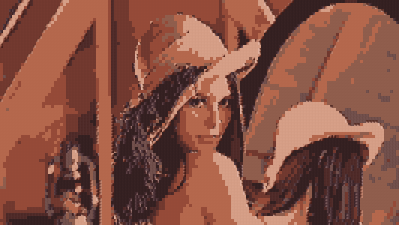
\includegraphics[width=12cm]{img/kmeans_2.png}
 \vspace{-0.0cm}
 \caption{Data: lenakolor3 Algorytm: k-średnich frameSz = 3 n = 20 iter = 10
}
\end{figure}

\begin{figure}[h!]
\centering
 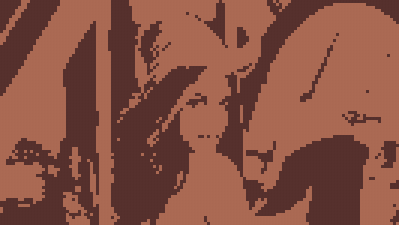
\includegraphics[width=12cm]{img/kmeans_4.png}
 \vspace{-0.0cm}
 \caption{Data: lenakolor3 Algorytm: k-średnich frameSz = 3 n = 2 iter = 30
}
\end{figure}

\newpage

\begin{figure}[h!]
\centering
 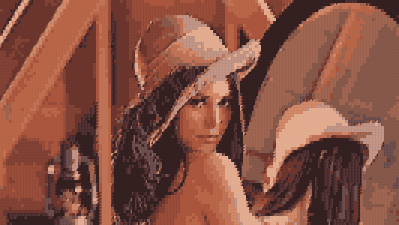
\includegraphics[width=12cm]{img/kohonen_4.png}
 \vspace{-0.0cm}
 \caption{Data: lenakolor3 Algorytm: kohonena frameSz = 3 n = 20 iter = 10000 mapRadius = 100 learningRate = 0.1 learningRate0 = 0.1
}
\end{figure}

\begin{figure}[h!]
\centering
 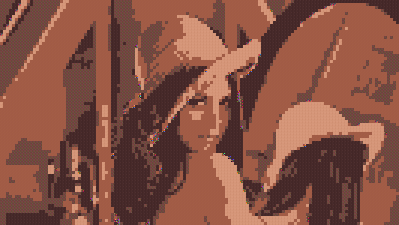
\includegraphics[width=12cm]{img/kohonen_5.png}
 \vspace{-0.0cm}
 \caption{Data: lenakolor3 Algorytm: kohonena frameSz = 3 n = 20 iter = 1000 mapRadius = 0.01 learningRate = 0.1 learningRate0 = 1
}
\end{figure}

\newpage

\begin{figure}[h!]
\centering
 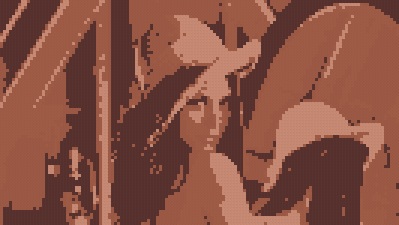
\includegraphics[width=12cm]{img/kohonen_6.png}
 \vspace{-0.0cm}
 \caption{Data: lenakolor3 Algorytm: kohonena frameSz = 3 n = 20 iter = 10000 mapRadius = 300 learningRate = 0.1 learningRate0 = 0.01
}
\end{figure}

\begin{figure}[h!]
\centering
 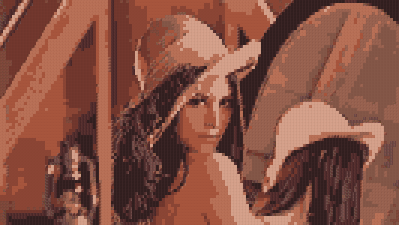
\includegraphics[width=12cm]{img/neural_1.png}
 \vspace{-0.0cm}
 \caption{Data: lenakolor3 Algorytm: gazu neuronowego frameSz = 3 n = 20 iter = 1000 mapRadius = 100 learningRate = 0.1 learningRate0 = 1
}
\end{figure}

\newpage

\begin{figure}[h!]
\centering
 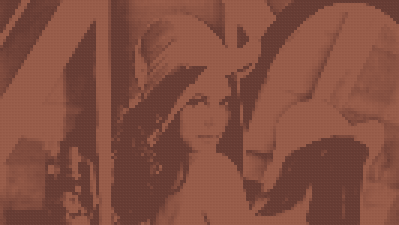
\includegraphics[width=12cm]{img/neural_3.png}
 \vspace{-0.0cm}
 \caption{Data: lenakolor3 Algorytm: gazu neuronowego frameSz = 3 n = 20 iter = 1000 mapRadius = 300 learningRate = 0.1 learningRate0  = 0.01
}
\end{figure}

\begin{figure}[h!]
\centering
 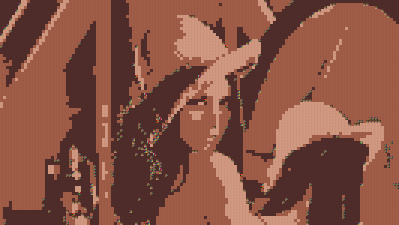
\includegraphics[width=12cm]{img/neural_4.png}
 \vspace{-0.0cm}
 \caption{Data: lenakolor3 Algorytm: gazu neuronowego frameSz = 3 n = 20 iter = 1000 mapRadius = 0.01 learningRate = 0.1 learningRate0  = 1
}
\end{figure}

\newpage

\begin{figure}[h!]
\centering
 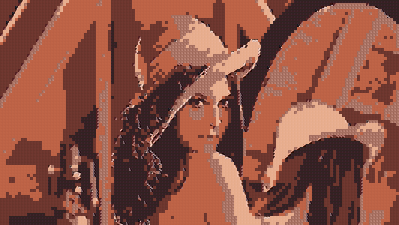
\includegraphics[width=12cm]{img/neural_5.png}
 \vspace{-0.0cm}
 \caption{Data: lenakolor3 Algorytm: gazu neuronowego frameSz = 3 n = 20 iter = 1000 mapRadius = 100 learningRate = 1.5 learningRate0  = 1
}
\end{figure}
}

\subsection{Porównanie podobieństwa obrazu wyjściowego z wejściowym}

\begin{figure}[h!]
 \centering
 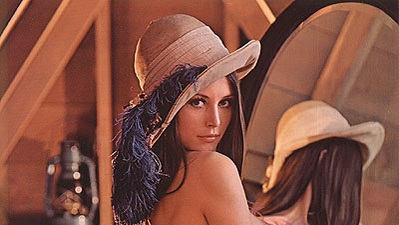
\includegraphics[width=12cm]{img/lenakolor3.jpg}
 \vspace{-0.3cm}
 \caption{Obrazek wejściowy
}
\end{figure}

\newpage

\begin{figure}[h!]
 \centering
 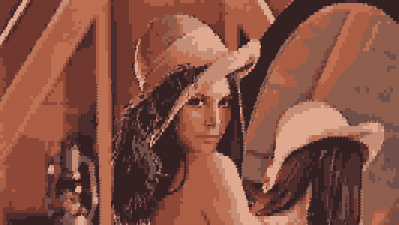
\includegraphics[width=12cm]{img/km1.png}
 \vspace{-0.3cm}
 \caption{Data: lenakolor3 Algorytm: k-średmich frameSz = 3 n = 20 iter = 20 procentowa różnica: 3.95%
}
\end{figure}

\begin{figure}[h!]
 \centering
 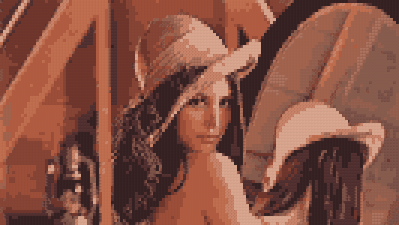
\includegraphics[width=12cm]{img/ng1.png}
 \vspace{-0.3cm}
 \caption{Data: lenakolor3 Algorytm: gazu neuronowego frameSz = 3 n = 20 iter = 2000 mapRadius = 50 learningRate = 0.05 learningRate0  = 1 procentowa różnica: 3.86
}
\end{figure}

\newpage

\begin{figure}[h!]
 \centering
 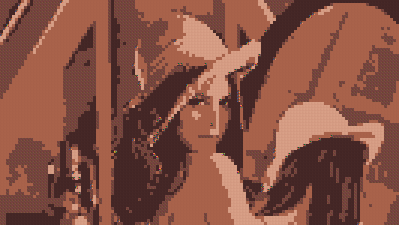
\includegraphics[width=12cm]{img/khn1.png}
 \vspace{-0.3cm}
 \caption{Data: lenakolor3 Algorytm: Kohonena frameSz = 3 n = 20 iter = 2000 mapRadius = 1 learningRate = 0.05 learningRate0  = 1 procentowa różnica: 5.72
}
\end{figure}

\begin{figure}[h!]
 \centering
 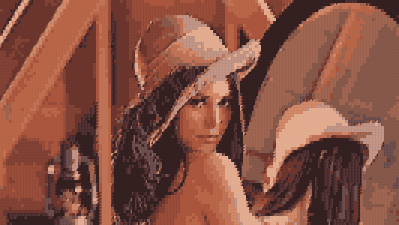
\includegraphics[width=12cm]{img/kohonen_4.png}
 \vspace{-0.3cm}
 \caption{Data: lenakolor3 Algorytm: Kohonena frameSz = 3 n = 20 iter = 10000 mapRadius = 1 learningRate = 0.1 learningRate0  = 1 procentowa różnica: 3.70
}
\end{figure}

\newpage

\begin{figure}[h!]
 \centering
 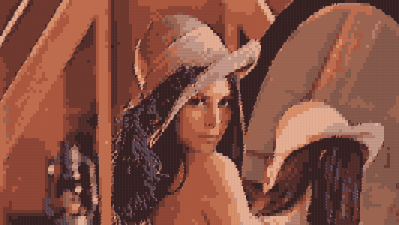
\includegraphics[width=12cm]{img/ng2.png}
 \vspace{-0.3cm}
 \caption{Data: lenakolor3 Algorytm: gazu neuronowego frameSz = 3 n = 20 iter = 10000 mapRadius = 50 learningRate = 0.1 learningRate0  = 1 procentowa różnica: 3.80
}
\end{figure}

\section{Dyskusja i wnioski}
\subsection{Algorytm k-średnich}
Algorytm k-średnich wymaga niewielkiej liczby iteracji aby osiągnąć satysfakcjonujące wyniki. Neurony nie są tutaj ze sobą powiązane, przemieszczenie jednego nie wpływa bezpośrednio na położenie sąsiednich. W przypadku tego algorytmu zbyt mała ilość iteracji może mieć wpływ na pogorszenie wyniku lub złe położenie początkowe neuronów jednak drugi czynnik jest minimalizowany poprzez losowanie początkowego położenia na podstawie rozkładu Gaussa.
\subsection{Algorytm Kohonena i gazu neuronowego}
Dla algorytmu Kohonena duże znaczenie mają początkowe parametry. Dla zbyt dużego promienia, który będzie stosunkowo wolno malał wszystkie neurony zbiegną się do środka ciężkości - Rys. 3). Prawidłowo przeprowadzony algorytm powinien przebiegać w dwóch etapach. W pierwszym promień sąsiedztwa i szybkość nauki powinny być stosunkowo duże tak aby sieć przesunęła się w kierunku skupisk danych. Drugim etapem jest wymodelowanie sieci dla okolicznych punktów. Tutaj promień sąsiedztwa i szybkość nauki są już niewielkie. Ze względu na to, że początkowe położenie neuronów obliczamy na postawie rozkładu Gaussa, pierwszy etap jest pomijalny. Z tego powodu dla Rys. 9 gdzie początkowy promień był niewielki uzyskano lepszy wynik niż dla Rys.10 gdzie promień był większy, co powodowało skupienie się neuronów do większych klastrów, natomiast mniejsze nie zostały uwzględnione przez co obrazek na Rys. 10 ma mniej szczegółów. \\
Algorytm gazu neuronowego działa najlepiej gdy promień sąsiedztwa obejmuje część sąsiednich neuronów - Rys 11. Promień sąsiedztwa nie jet tutaj tak inwazyjny i nie powoduje tak dużego przyciągania się neuronów znajdującego się wewnątrz promienia, a umożliwia elastyczne dostosowywanie się sieci.  \\
Dla obu algorytmów parametr szybkości uczenia powinien być dość mały. Dla większych wartości neurony są zbyt mocno przyciągane do wybranego punktu danych. Na Rys. 14 widać, że obrazek ma większy kontrast niż Rys. 11 co wynika ze zbyt dużej wartości parametru szybkości uczenia. \\
Algorytmy Kohonena i gazu neuronowego wymagają większej ilości czasu, ale dla tej samej liczby neuronów pozwalają osiągnąć lepsze wyniki niż metodą k-średnich - Rys.16-20. Algorytm gazu neuronowego pozwala osiągnąć lepsze wyniki dla mniejszej ilości iteracji w porównaniu z algorytmem Kohonena - Rys.17-18 ale algorytm Kohonena ostatecznie dla dużej ilości iteracji daje najlepsze wyniki - Rys.19-20.
}

\end{document}
